\documentclass[]{bioinfo}
\copyrightyear{2009}
\pubyear{2009}

% - - - - - - - - - - - - - - - - - - - - - - - - - - - - - - - - 
% User-specific packages, macros, and settings
% - - - - - - - - - - - - - - - - - - - - - - - - - - - - - - - - 
\usepackage{amsmath} 
\usepackage{amsfonts} 
\usepackage{xspace}
\usepackage{graphicx}
\usepackage{timestamp} 

\newcommand{\gAA}{\textnormal{AA}\xspace}
\newcommand{\gAB}{\textnormal{AB}\xspace}
\newcommand{\gBB}{\textnormal{BB}\xspace}
\newcommand{\eps}{\varepsilon\xspace}
\newcommand{\pkg}[1]{\textit{#1}\xspace}
\newcommand{\CN}{\textnormal{CN}\xspace}
\newcommand{\kb}{\textnormal{kb}\xspace}
\newcommand{\GWSSixf}{GenomeWideSNP\_6\xspace}
%\newcommand{\CP}{\ensuremath{\textnormal{CP}}\xspace}
%\newcommand{\CPs}{\ensuremath{\textnormal{CPs}}\xspace}
\newcommand{\CP}{\ensuremath{\textnormal{change point}}\xspace}
\newcommand{\CPs}{\ensuremath{\textnormal{change points}}\xspace}

% Comment the 2nd row to highlight updates
% \newcommand{\updated}[2][red]{{\color{#1}{#2}}\xspace}
% \renewcommand{\updated}[2][red]{#2\xspace}

\graphicspath{{figures/col/}}



\begin{document}
\firstpage{1}

\title[TumorBoost]{TumorBoost: A single-sample method for calibrating allele-specific tumor copy numbers in paired tumor-normal designs}
\author[Bengtsson et al.]{Henrik Bengtsson\,$^{\rm a}$\footnote{To whom correspondence should be addressed}, Pierre Neuvial\,$^{\rm a}$, Terence P. Speed\,$^{\rm a,b}$}
\address{
  $^{\rm a}$ Department of Statistics, University of California, Berkeley, USA.
  $^{\rm b}$ Bioinformatics Division, Walter \& Eliza Hall Institute of Medical Research, Parkville, Australia.
} 

\history{Version: \timestamp; Received on March NN, 2009}

\editor{Associate Editor: XXX}

\maketitle

%%%%%%%%%%%%%%%%%%%%%%%%%%%%%%%%%%%%%%%%%%%%%%%%%%%%%%%%%%%%%%%%%%%%%%%%%%%
% ABSTRACT
%%%%%%%%%%%%%%%%%%%%%%%%%%%%%%%%%%%%%%%%%%%%%%%%%%%%%%%%%%%%%%%%%%%%%%%%%%%
\begin{abstract}
\section{Motivation:}
The availability of high-quality allele-specific copy number estimates for a tumor tissue allows for improved genotype and loss-of-heterozygosity calls

\section{Results:}
We propose a single-sample method for calibrating allele-specific copy number (ASCN) estimates of a tumor based on ASCN estimates of a paired normal.  
The method applies to any paired tumor-normal copy-number estimates regardless of technology and generation.
Here we demonstrate the method using tumor-normal pairs from the Cancer Genome Atlas (TCGA) project. 
We show that the calibrated ASCN estimates for the tumor are significantly better than the ones obtained if no paired normal is available.
Combined with single-array preprocessing methods, such as CRMA~v2, we conclude that for tumor tissues, ASCN estimates with high precisions can be obtained from a single pair of tumor-normal hybridizations.

\section{Availability:}
A single-sample bounded-memory implementation is available in \pkg{aroma.cn}.


\section{Contact:} 
\href{hb@stat.berkeley.edu}{hb@stat.berkeley.edu}
\end{abstract}


%%%%%%%%%%%%%%%%%%%%%%%%%%%%%%%%%%%%%%%%%%%%%%%%%%%%%%%%%%%%%%%%%%%%%%%%%%%
% INTRODUCTION
%%%%%%%%%%%%%%%%%%%%%%%%%%%%%%%%%%%%%%%%%%%%%%%%%%%%%%%%%%%%%%%%%%%%%%%%%%%
\section{Introduction}
\label{secBackground}

The Cancer Genome Atlas (TCGA) project~\citep{CollinsBarker_2007,TCGA_2008c} is a collaborative initiative to better understand cancer using existing large-scale whole-genome technologies.  Several tumor types are or are planned to be studied, including brain cancer (glioblastoma multiforma; GBM), ovarian cancer and lung cancer.  Several of these tumors are often agressive and requires immediate treatments to slow or stop the progression of the tumor growth.

[...]

In this paper we present a method for calibrating the allele-specific copy-number estimates (ASCNs) of a tumor tissue given ASCNs of matched normal tissue or blood extract.  The method does not require external references and it is only the relative ASCNs that are calibrated, that is, the total CN estimates are not adjusted.

The realization of a single-sample method has several implications:
(i) Each tumor-normal pair can be analyzed immediately without needing reference samples.
(ii) Samples can be processed in parallel on different hosts/processors making it possible to decrease the processing time of large data sets.
(iii) There is no need to reprocess a sample when new samples are produced, which further saves time and computational resources.
Furthermore, (iv) the decision to filter out poor samples can be made later, because a poor sample will not affect the processing of other samples.
More importantly, a single-sample method is
(v) more practical for applied medical diagnostics, because individual patients can be analyzed at once, even when they come singly rather than in batches.  This may otherwise be a limiting factor in projects with a larger number of samples.

The outline of this paper is as follows. 
In Methods, we describe the underlying model and algorithm for the calibration method.
In Results, we show that the signal-to-noise ratios (SNRs) of the calibrated ASCNs are significantly larger than corresponding non-calibrated estimates.
In Discussion, we conclude the study, discuss potential limitations, ..., and give future research directions.


%%%%%%%%%%%%%%%%%%%%%%%%%%%%%%%%%%%%%%%%%%%%%%%%%%%%%%%%%%%%%%%%%%%%%%%%%%%
% METHODS
%%%%%%%%%%%%%%%%%%%%%%%%%%%%%%%%%%%%%%%%%%%%%%%%%%%%%%%%%%%%%%%%%%%%%%%%%%%
\begin{methods}
\section{Methods}



%--------------------------------------------------------------------------
% DATA SET
%--------------------------------------------------------------------------
\subsection{Data set}
For this study, we used data from the TCGA project.  From the DCC data portal, we downloaded (Jan 2009) raw data (Level~1; CEL files) for a set of GBM tumor-normal pairs.
For the purpose of illustrating our method, we will focus mainly on sample TCGA-02-0104 (vials 01A vs 10A), because it has a large number of CN aberrations on Chr~3 at different mean levels.


\subsubsection{Allele-specific SNP signals and allele B fractions}
The allele~B fraction~\cite{PeifferD_etal_2006} for SNP $j=1,\ldots,J$ in the nnormal ($N$) tissue is defined as:
\begin{equation}
  \beta_{N,j} = \frac{\theta_{N,j,A}}{\theta_{N,j}},
  \label{eqnCnLogRatio}
\end{equation}
where $\theta_{N,j} = \theta_{N,j,A} + \theta_{N,j,B}$ is the non-polymorphic signal at locus $j$.
TODO: DEFINE $(\theta_{N,j,A}, \theta_{N,j,B})$.
For a diploid SNP $j$, for which the genotype is either AA, AB or BB, we expect the allele~B fraction $\beta_{N,j}$ to be fall close to $0$, $1/2$, or $1$, respectively.
The allele~B fraction $\beta_{T,j}$ for the tumor ($T$) tissue/blood extract is defined analoguously. Because we cannot expected a SNP in a tumor to be diploid at any random SNP, we cannot make any prediction on where $\beta_{T,j}$ falls.

For a tumor-normal pair, we observe $(\beta_{N,j}, \beta_{T,j})$ at each SNP $j$.

\subsubsection{Model for allele~B fraction signals}
Consider a SNP $j$ that is diploid in the normal tissue.  
Let the true genotype be denoted by the true allele~B fraction $\mu_{N,j}$ with possible states $\{0,1/2,1\}$ corresponding to genotypes $\{\gAA,\gAB,\gBB\}$.

Based on this, for SNP $j$ we model the observed allele~B fraction for the tumor and the normal pair as:
\begin{equation}
  \beta_{T,j} = \mu_{T,j} + \delta_{j} + \eps_{T,j},\\
  \beta_{N,j} = \mu_{N,j} + \delta_{j} + \eps_{N,j},
  \label{eqnFracBModel}
\end{equation}
where $\delta_{j}$ is a SNP-specific effect and $\eps_{T,j}$ and $\eps_{N,j}$ are independent zero-mean error terms.

An estimate of $\mu_{T,j}$ is then:
\begin{equation}
  \hat{\mu_{T,j}} = \beta_{T,j} - \hat{\delta_{j}},
  \label{eqnTumorBoostEstimate}
\end{equation}
where $\hat{\delta_{j}} = \beta_{N,j} - \hat{\mu_{N,j}}$ and $\hat{\mu_{N,j}}$ is an estimate of the allele~B fraction of the normal, i.e. an estimate of the normal genotype of SNP $j$.


%--------------------------------------------------------------------------
% EVALUATION METHODS
%--------------------------------------------------------------------------
\subsection{Evaluation}
\label{secEvaluation}



\subsection{Algorithm and implementation}
The TumorBoost calibration method is available in R~\citep{RDevel_2008} package \pkg{aroma.cn} part of the \pkg{aroma.affymetrix} framework~\citep{BengtssonH_etal_2008b}.  The  method is designed and implemented to have bounded-memory usage, regardless of the number of samples/arrays processed. 
Furthermore, the complexity of the algorithm is linear in the number of loci ($J$).
Since it is a single-sample method, the tumor-normal pairs can be calibrated in parallel on multiple hosts/processors.
The method applies estimates obtained by SNP technology.
\end{methods}


 
%%%%%%%%%%%%%%%%%%%%%%%%%%%%%%%%%%%%%%%%%%%%%%%%%%%%%%%%%%%%%%%%%%%%%%%%%%%
% RESULTS
%%%%%%%%%%%%%%%%%%%%%%%%%%%%%%%%%%%%%%%%%%%%%%%%%%%%%%%%%%%%%%%%%%%%%%%%%%%
\section{Results}
\label{secResults}

\subsection{Allele~B fraction before and after calibration}
\begin{figure}[!tpbh]
\begin{center}
  \resizebox{0.96\columnwidth}{!}{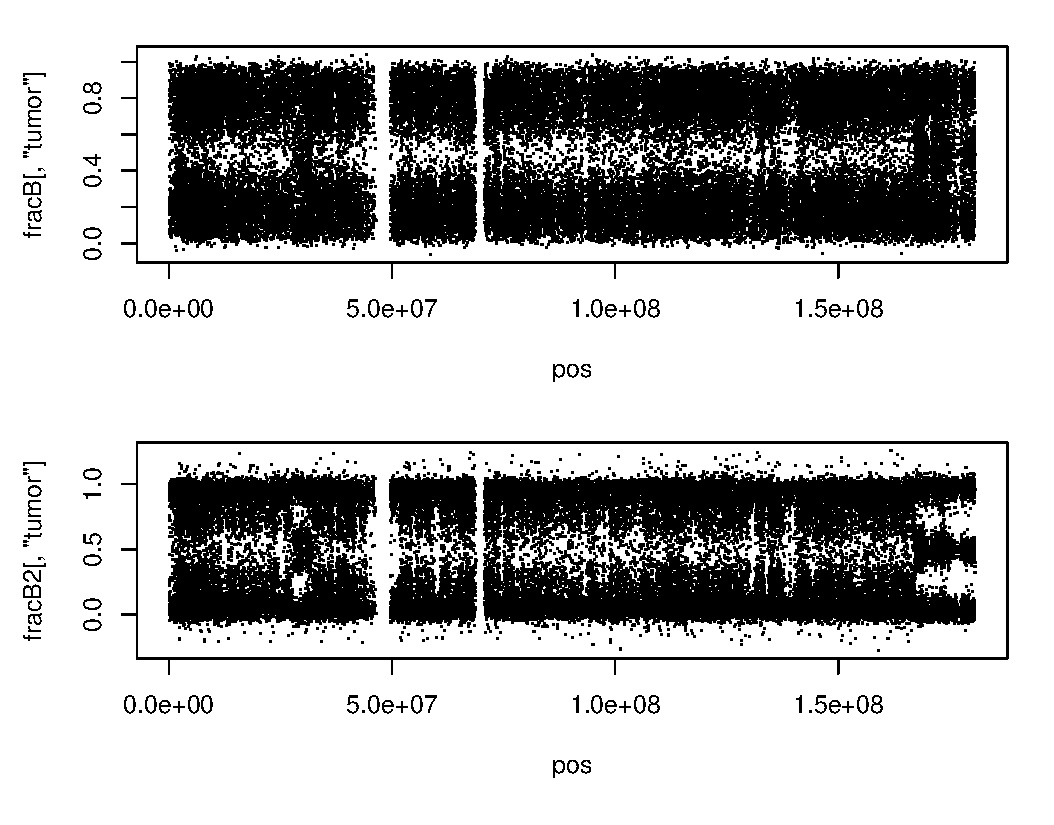
\includegraphics{TCGA-02-0069,tumor,Chr05,fracB,beforeAndAfter}}%
\end{center}
 \caption{
 }
 \label{figROCs}
\end{figure}

\begin{figure}[!tpbh]
\begin{center}
  \resizebox{0.96\columnwidth}{!}{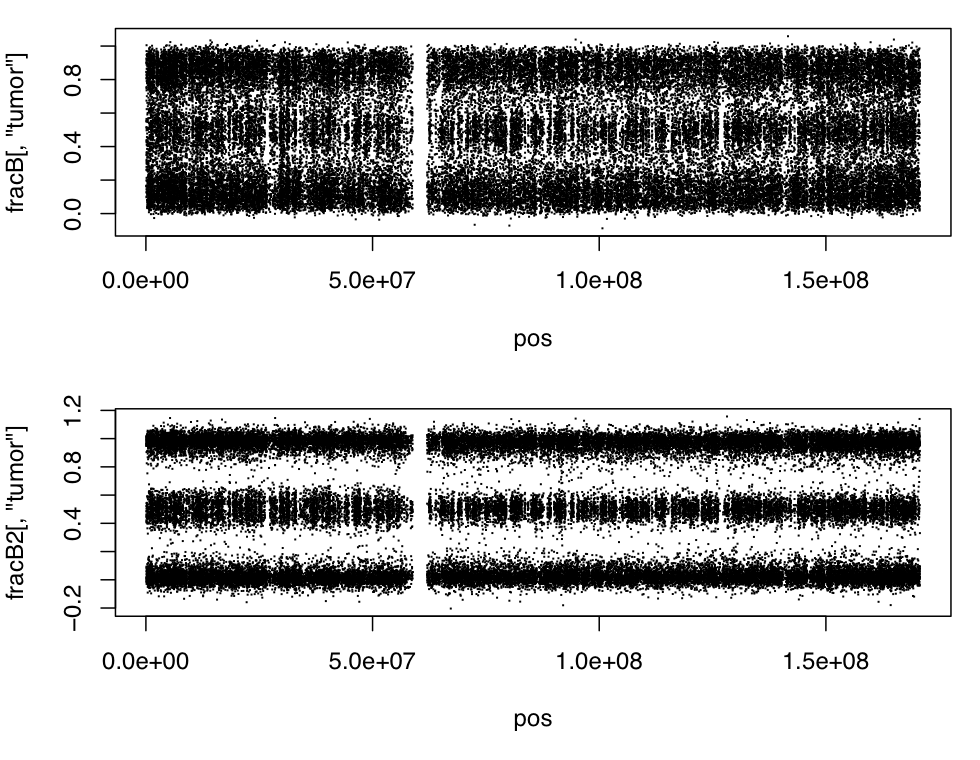
\includegraphics{TCGA-02-0069,tumor,Chr06,fracB,beforeAndAfter}}%
\end{center}
 \caption{
 }
 \label{figROCs}
\end{figure}


\begin{figure}[!tpbh]
\begin{center}
  \resizebox{0.96\columnwidth}{!}{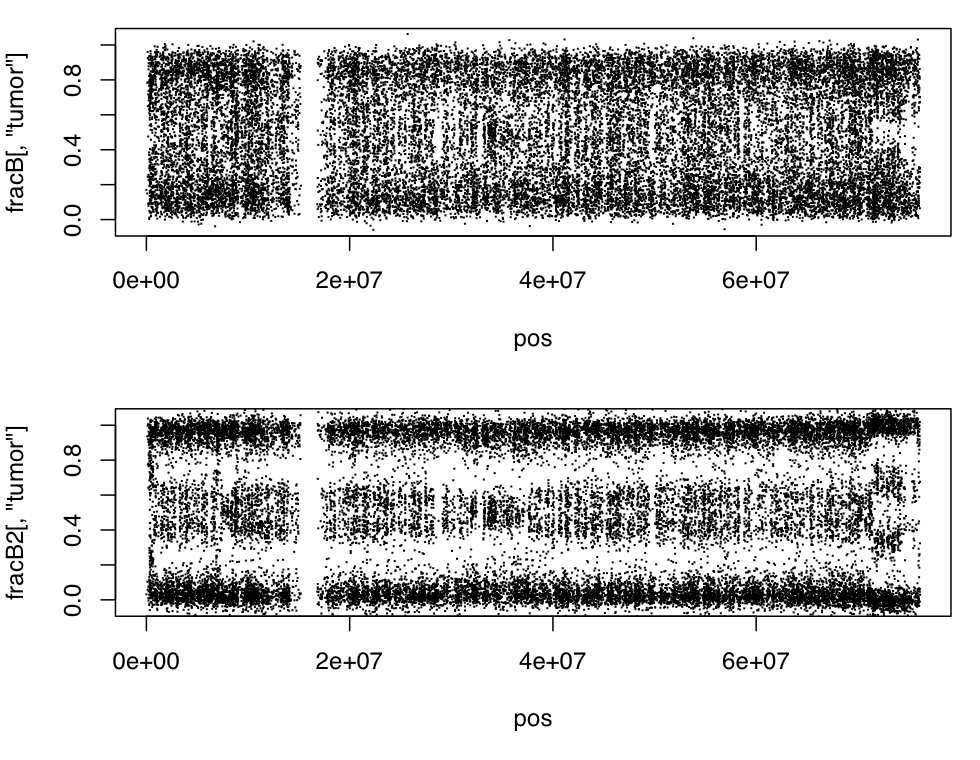
\includegraphics{TCGA-02-0069,tumor,Chr18,fracB,beforeAndAfter}}%
\end{center}
 \caption{
 }
 \label{figROCs}
\end{figure}



%%%%%%%%%%%%%%%%%%%%%%%%%%%%%%%%%%%%%%%%%%%%%%%%%%%%%%%%%%%%%%%%%%%%%%%%%%%
% DISCUSSION
%%%%%%%%%%%%%%%%%%%%%%%%%%%%%%%%%%%%%%%%%%%%%%%%%%%%%%%%%%%%%%%%%%%%%%%%%%%
\section{Discussion}
\label{secDiscussion}




%%%%%%%%%%%%%%%%%%%%%%%%%%%%%%%%%%%%%%%%%%%%%%%%%%%%%%%%%%%%%%%%%%%%%%%%%%%
% ACKNOWLEDGEMENTS
%%%%%%%%%%%%%%%%%%%%%%%%%%%%%%%%%%%%%%%%%%%%%%%%%%%%%%%%%%%%%%%%%%%%%%%%%%%
\section*{Acknowledgements}
We gratefully acknowledge the TCGA Consortium and all its members for the TCGA Project initiative, for providing samples, tissues, data processing, and making data and results available.

\emph{Funding}: NCI grant U24 CA126551.

\emph{Conflict of interest}: none declared.


%%%%%%%%%%%%%%%%%%%%%%%%%%%%%%%%%%%%%%%%%%%%%%%%%%%%%%%%%%%%%%%%%%%%%%%%%%%
% REFERENCES
%%%%%%%%%%%%%%%%%%%%%%%%%%%%%%%%%%%%%%%%%%%%%%%%%%%%%%%%%%%%%%%%%%%%%%%%%%%
\begin{methods}
\bibliography{bioinformatics-journals-abbr,hb-at-maths.lth.se}
\bibliographystyle{natbib}
\end{methods}
 
%\begin{thebibliography}{}
%\end{thebibliography} 

\end{document}
